\section{The ATM benchmark}
An ATM is a computerized system that provides financial services for users in 
a public space. 
%\textit{Automatic Teller Machine} (ATM) is a computerized telecommunication device
%that provides services to access to financial transactions in a public space without
%the need for a cashier, human clerk or bank teller.
Figure~\ref{fig:atm_bip} shows a structured BIP model of an ATM system adapted from the
description provided in~\cite{atm}.
The system is composed of four atomic components: (1) the User, (2) the ATM, (3) the Bank Validation 
and (4) the Bank Transaction. It is the job of the ATM component to handle all interactions between the 
users and the bank. No communication between the users and the bank is allowed. 
%The structural BIP model of an ATM system \cite{atm} is presented in Figure \ref{fig:atm_bip}.
%The system is composed of the following components: User, ATM (modeling a cash dispenser)
%and Bank (modeling some aspects of bank operation). User and Bank interact only with ATM,
%but not with each other.
\begin{figure}[bt]
 \centering
  %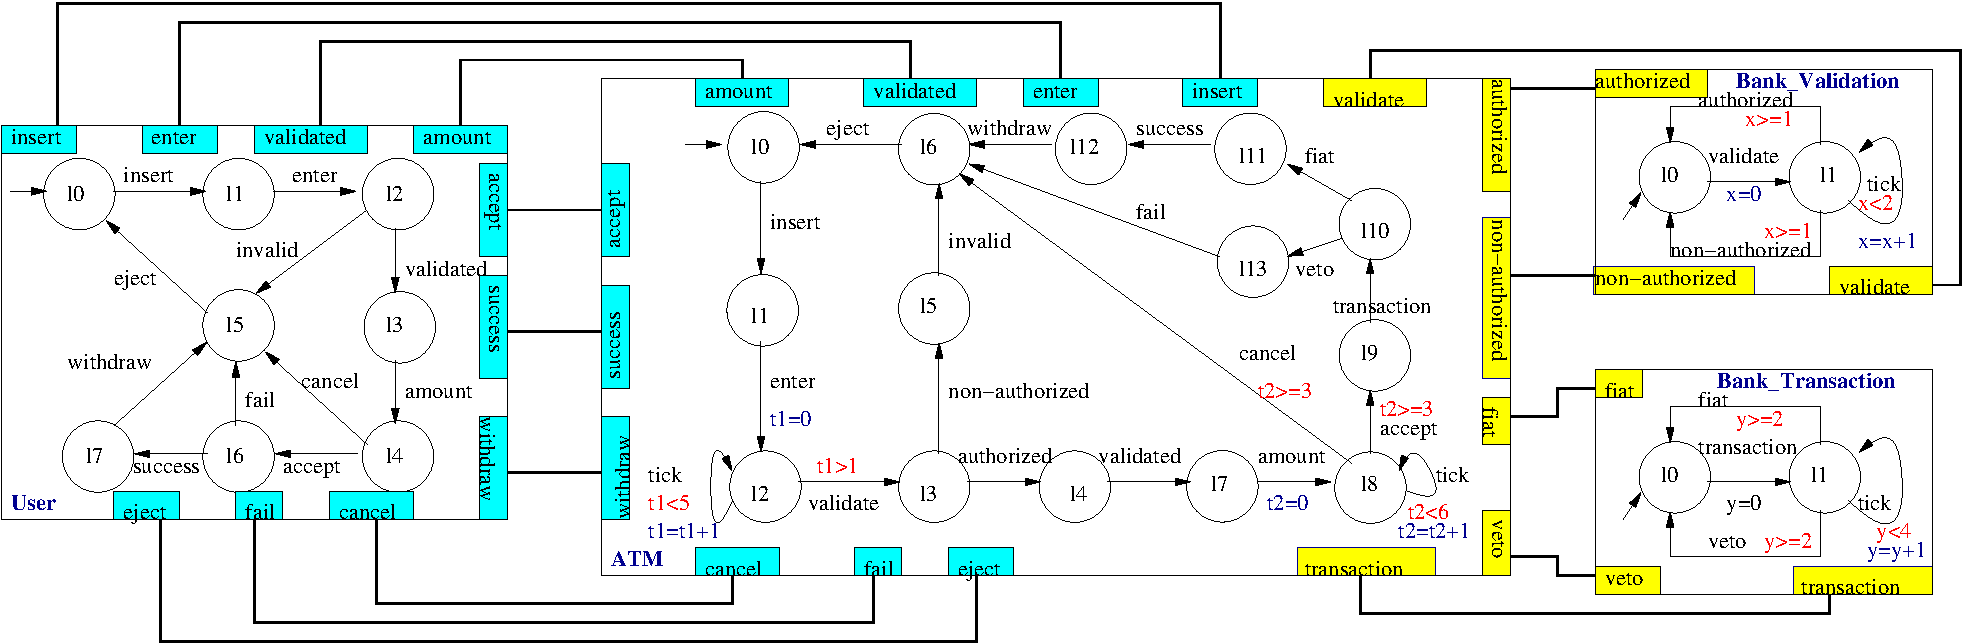
\includegraphics[width=1.0\textwidth]{figures/atm_bip.pdf}
  \resizebox{1.0\textwidth}{!}{
       \input{figures/atm_bip.pdftex_t}
  }
  \caption{Modeling of ATM system in BIP} \vspace*{-0.5cm}
  \label{fig:atm_bip}
% \end{center}
\end{figure}

The ATM starts from an idle location and waits for the user to insert his card 
and enter the confidential code. The user has $5$ time units
to enter the code before the counter expires and the card is ejected by the ATM. 
Once the code is entered, the ATM checks with the bank validation unit for 
the correctness of the code. If the code is invalid, the card is ejected
and no transaction occurs. If the code is valid, the ATM waits for the user to enter
the desired amount of money for the transaction. The time-out for entering the amount 
of money is of $6$ time units. 

Once the user enters the desired transaction amount, the ATM checks with the bank whether 
the transaction is allowed or not by communicating with the bank transaction unit.
If the transaction is approved, the money is transferred to the user and the card is ejected. 
If the transaction is rejected, the user is notified and the card is ejected. In all cases, 
the ATM goes back to the idle location waiting for any additional users. 
In our model, we assume the presence of a single bank and multiple ATMs and users. 

\begin{table}[tb]
\caption{ATM results}
\centering
\begin{tabular}{|c|c|c|c|c|c|c|c|c|c|}
\cline {2-10}
\multicolumn{1}{c|}{} &  \multicolumn{3}{c|}{Original} & \multicolumn{3}{c|}{After reduction} &  \multicolumn{3}{c|}{Time(s)} \\ \hline
ATMs & lat & and & lev & lat & and & lev & Ver. & Total& NuSMV \\ \hline
2 & 78 & 2308 & 125 & 37 & 552 & 25 & 21.83 & 26.1 & 1.4\\ \hline
3 & 102 & 3689 & 197 & 50 & 804 & 29 & 32.65 & 38.87 & 142.6 \\ \hline
4 & 146 & 5669 & 234 & 63 & 1036 & 29 & 590  & 597 & 3361 \\ \hline
\end{tabular}
\label{tb:bip:atm}
\end{table}

Table~\ref{tb:bip:atm} shows the improvement obtained by using \biptool{}
to verify the deadlock freedom of the ATM system, as compared to using the
NuSMV model checker~\cite{nusmv}.
The first column of the table shows the number of clients and ATMs in the system.
Columns \cci{lat}, \cci{and} and \cci{lev} present the number 
of latches, AND gates and logic levels in the AIG generated by \biptool{} before
and after applying reduction techniques, respectively.
We report on the verification time taken by the ABC solver to check the 
generated AIG, and the total taken to perform both synthesis (reduction) 
and verification, in addition to the time taken by NuSMV to perform verification.

With the increase in the number of users and ATMs in the system, \biptool{}  
outperforms NuSMV in terms of total verification time, reaching a speedup 
of $5.6$ for 4 users and ATMs. Additionally, \biptool{} allows developers
to make use of several reduction techniques that are able to reach an 
average of $50\%$ reduction in the size of the AIG. Note that for $2$ ATMs 
and users, NuSMV outperforms \biptool{}. This is due to the fact that when 
performing verification, ABC tries multiple verification and reduction 
algorithms before reaching a conclusive result. However, the advantage 
that \biptool{} presents can be clearly seen for larger number of ATMs and 
users. 